% ============================================================
%  ECE284 Final Project Report
%  Format: ACM acmtog (Large 2-column) — matches the provided template PDF.
%  To switch to sigconf (conference proceedings), change acmtog → sigconf.
%  Target: 7–10 pages.
% ============================================================
\documentclass[acmtog]{acmart}

% ------ Packages ------
\usepackage{booktabs}       % \toprule / \midrule / \bottomrule
\usepackage{graphicx}
\usepackage{multirow}
\usepackage{xcolor}
% amssymb is already loaded by acmart — do not re-load it
% \checkmark is available via amssymb which acmart imports internally
\usepackage{microtype}      % Better text spacing in 2-col

% ------ Suppress ACM boilerplate for course submission ------
\settopmatter{printacmref=false}
\renewcommand\footnotetextcopyrightpermission[1]{}
\AtBeginDocument{\pagestyle{plain}}

% ------ Convenience: placeholder box for missing figures ------
% Usage: \missingfig{width}{label}{script to run}
\newcommand{\missingfig}[3]{%
  \fbox{\begin{minipage}{#1}\centering\vspace{0.8em}
    {\small\textcolor{red}{[Figure missing --- run \texttt{#3}]}}\\[0.4em]
    {\footnotesize\textit{#2}}\vspace{0.8em}
  \end{minipage}}%
}

% ============================================================
\title{Proof-of-Concept Lesional Skin Classification with\\
       IDC Wearable Sensors under Data Scarcity}

\author{[Juqy Chen]}
\affiliation{
  \institution{University of California San Diego}
  \department{Electrical and Computer Engineering}
}
\email{[juc052]@ucsd.edu}

% ============================================================
\begin{document}

\begin{abstract}
Continuous monitoring of Atopic dermatitis (AD) through wearable interdigitated capacitive (IDC) sensors offers a non-invasive physiological proxy for skin barrier integrity. However, existing datasets present a severe data-scarcity challenge; the only publicly available corpus contains just 13 patients, each providing only two 30-second traces (one lesional and one non-lesional). I present a proof-of-concept
classification pipeline on this corpus and address two testable questions:
whether a short trace prefix captures sufficient discriminative signal, and
whether a machine learning model can generalize across unseen patients without relying on population-level thresholding. Six statistical features (mean, median, slope, std, range, skewness) extracted from raw traces and normalized with feature-level z-score inside each LOSO fold yield a LinearSVC with GroupKFold AUC of 0.822 and
pairwise ranking accuracy of 13/13 held-out patients. A compact 1D CNN with
Global Average Pooling matches and slightly exceeds the SVM (GKF AUC 0.871), confirming that the discriminative signal is the per-site mean capacitance level rather than complex temporal dynamics. Self-supervised pretraining on domain-adjacent electrodermal activity (EDA) data from WESAD followed by frozen-layer transfer (Track B) yields GKF AUC 0.827 --- above the SVM but below the from-scratch CNN --- indicating that the EDA--IDC sensor physics gap limits transfer benefit at $N{=}26$ traces. Finally, an analysis of measurement duration reveals that early-trace classification advantages stem from a data-quality confound—specifically, forward-filling in several traces—rather than a genuine clinical advantage of shorter measurement durations. These results confirm the viability of personalized, intra-individual tracking for AD, though population-level validation demands a substantially larger and more complete dataset.

\end{abstract}

\keywords{atopic dermatitis, interdigitated capacitive sensor, data scarcity, time-series classification}

\maketitle

% ============================================================
\section{Motivation}\label{sec:motivation}
Atopic dermatitis (AD) is one of the most prevalent chronic inflammatory skin
diseases, affecting approximately 15--20\% of children and 2--10\% of adults
worldwide \cite{sanchez2019atopic}. Characterized by persistent skin barrier
dysfunction, intense itchiness, and recurrent flares, AD requires ongoing
monitoring to assess disease activity and guide treatment. Traditional clinical
assessment relies on in-person evaluations that lack longitudinal tracking between
clinic visits, and many patients struggle to convey their condition precisely to
clinicians. Even the standard clinical score, the Eczema Area and Severity Index
(EASI), shows only moderate inter-observer reliability \cite{khan2024skin}; combined
with the day-to-day fluctuation of AD severity, this makes a single clinic visit an
unreliable snapshot and motivates continuous, at-home monitoring.
 
Among wearable approaches, behavioral itch sensing (for example, wrist actigraphy for
scratch) is the best-evidenced family, but it captures a behavioral proxy downstream
of the disease; barrier-function capacitance instead measures the physiological state
of the skin directly and continuously, making longitudinal physiological tracking
possible. This motivates the focus of this work on the interdigitated capacitive
(IDC) sensor of Todorov et al.\ \cite{todorov2025wearable}. By measuring the dielectric
permittivity of skin at the sensor interface, IDC devices provide a proxy for skin
hydration and barrier integrity --- both key indicators of AD severity. The system
samples skin capacitance at 1\,Hz over a 30-second contact window, producing a compact
time-series trace per measurement site. Non-lesional skin consistently exhibits higher
capacitance than lesional skin due to differences in stratum corneum hydration, and the
sensor captures this contrast without any chemical reagents or clinical-grade equipment.
 
Despite this promise, publicly available IDC datasets for AD patients remain
extremely limited. To our knowledge, the Todorov et al.\ \cite{todorov2025wearable}
corpus is the only public dataset pairing IDC traces with AD lesional labels:
13 patients, each contributing one 30-second lesional trace and one non-lesional
trace (26 traces total). No second IDC-on-AD dataset exists for cross-dataset
validation. This extreme data scarcity --- $N{=}13$ patients, binary per-patient
labeling --- makes standard supervised learning difficult to apply and motivates
a rigorous evaluation strategy that prevents patient identity leakage.
 
Within this constraint, two testable questions drive the experimental design.
(1) Is a short trace prefix sufficient for classification, or does extending the
measurement window improve discrimination? Todorov et al.\ \cite{todorov2025wearable}
established lesional/non-lesional separability and 30-second stability but did not test
whether fewer than 30 seconds suffice. They report a slight capacitance drift in the
first 5--10 seconds, attributed to the skin conforming around the sensor; later samples
may therefore carry the genuine physiological signal, though the reverse is also possible
if some traces contain only a few seconds of real data before forward-filling.
(2) Can a model trained on a subset of patients correctly rank lesional above
non-lesional skin for an entirely unseen patient, without any population-wide threshold?
This directly tests the intra-individual tracking capability that Todorov et al.\ highlight
as the practical use case for their sensor, which they did not quantify across patients.
 
% ============================================================
\section{Related Work}\label{sec:related}
 
\subsection*{The landscape of AD wearable sensing}
Khan et al.\ \cite{khan2024skin} present a systematic review of AD wearables and group
them into three families: behavioral/itch sensing (actigraphy, smartwatches), surface
barrier-function sensing (e-textiles, capacitance, TEWL), and intradermal sensing
(microneedles, ISF biomarkers). Behavioral itch sensing is the best-evidenced family,
but the IDC sensor used in this work belongs to the surface barrier-function family,
which targets skin pathology more directly. Across the field, few of the surveyed
systems release public data, so a publicly available, labeled IDC corpus is a
precondition for the supervised learning pursued here.
 
\subsection*{IDC sensors and skin capacitance}
Todorov et al.\ \cite{todorov2025wearable} introduced a printed IDC sensor for
wearable AD monitoring and demonstrated that non-lesional skin capacitance
consistently exceeds lesional capacitance at the individual patient level.
They report Corneometer correlations confirming that capacitance tracks skin
hydration, and note explicitly that a population-wide threshold cannot
distinguish lesional from non-lesional skin across patients due to inter-patient
baseline variation. Our work formalizes this observation through leave-one-subject-out
cross-validation and adds a quantitative measure of cross-patient generalization.
No second public IDC-on-AD-patients dataset exists; cross-dataset comparison was
out of scope as available alternatives use different sensor modalities.
 
\subsection*{Machine learning on small AD datasets}
Xing et al.\ \cite{xing2024nocturnal} offer a methodological parallel from a different
sensing modality: wrist actigraphy for nocturnal scratch detection in a cohort of seven
subjects, five of them with AD. Because the signal (limb motion) and target (scratch
behavior) differ fundamentally from skin capacitance, no signal-level comparison with
the IDC data is meaningful; the relevance is the modeling regime. On the same small
dataset they compared a feature-engineering gradient-boosting model against a 1D CNN,
and the gradient-boosting model achieved a higher minority-class F1 (0.45 vs.\ 0.39),
which they attribute to the small sample favoring a lower-capacity model with fewer
hyperparameters. This is consistent with the data-scarcity framing of our
SVM-versus-CNN comparison (Section~\ref{sec:cnn_a}): rather than the deep model
realizing its usual advantage, the two paradigms converge, indicating that AD datasets
of this size do not yet justify the added capacity of end-to-end deep learning.

% ============================================================
\section{Project Aim}\label{sec:aim}
This work pursues three concrete aims within the data-scarcity constraint of the
Todorov et al.\ \cite{todorov2025wearable} corpus. All results are framed as
proof-of-concept findings on $N{=}13$ patients and are not intended as clinical validation.

\begin{enumerate}
  \item \textbf{Replication.} Reproduce the per-patient non-lesional $>$ lesional
        capacitance ordering reported in Todorov et al.\ Fig.\ 9(a), confirming
        dataset integrity and establishing the baseline visual separation.
  \item \textbf{Cross-patient generalization.} Quantify the gap between
        intra-individual tracking accuracy (LOSO pairwise ranking) and
        population-level threshold accuracy, and establish GroupKFold AUC as
        the honest discriminability metric under data scarcity.
  \item \textbf{End-to-end learning under scarcity.} Compare a six-feature
        LinearSVC against a compact 1D CNN (Track A, from-scratch) to test whether
        temporal modeling adds value beyond mean-level statistics, and assess
        whether self-supervised EDA pretraining followed by frozen-layer transfer
        (Track B) can improve on the from-scratch CNN at $N{=}26$ traces.
\end{enumerate}

% ============================================================
\section{Methodology}\label{sec:methodology}

\subsection{Dataset}
The dataset was introduced by Todorov et al.\ \cite{todorov2025wearable}. Thirteen
AD patients each contributed two 30-second IDC capacitance traces sampled at 1\,Hz
(30 samples per trace): one from a lesional site and one from a non-lesional site,
yielding 26 traces in total. Raw traces are loaded from CSV files; within-patient
missing values are forward-filled. At least three patients (S-02, S-03, S-04) have
genuine capacitance signal only in approximately the first 10 seconds; subsequent
samples are forward-filled constants from the last valid measurement. This
data-completeness confound is directly relevant to the window-length experiment
(Section~\ref{sec:stage4}) and is discussed further in Section~\ref{sec:discussion}.

\subsection{Evaluation Framework}\label{sec:eval}
Because every experiment below uses the same protocol, it is defined once here.
Three complementary views are reported throughout. \textit{LOSO} (13 folds, one
patient held out per fold) is the primary evaluation; because each fold contains
exactly one lesional and one non-lesional test sample, the per-fold AUC collapses
to a binary ranking indicator, so its mean across folds is a pairwise ranking
accuracy rather than a graded ROC area. \textit{GroupKFold} ($n{=}5$) assigns
2--3 patients to each test fold (4--6 samples), yielding a genuinely graded
per-fold AUC with lower fold-to-fold variance; this is the headline
discriminability metric. \textit{Pooled-LOSO AUC} concatenates all 26 LOSO test
scores into a single ROC curve; following Airola et al.\ \cite{airola2011comparison},
pooled leave-one-out AUC is a negatively biased estimator of true discriminability,
so it is reported only as a reference check. To prevent patient-identity leakage,
all feature scalers and baseline estimators are fit on training-fold data only,
with held-out patients receiving a training global-mean fallback.

\subsection{Feature Extraction (Stage 2)}
Six statistical features are extracted per trace: mean, standard deviation, median,
range (max$-$min), slope (ordinary least squares linear regression coefficient over
time), and skewness. 

% reasoning for the six features (independent of the review): summary statistics are a standard,
% low-variance representation for very short series (30 samples). The six capture level (mean,
% median), spread (std, range), trend (slope), and asymmetry (skewness); Stage 2 RF importances
% (Table~\ref{tab:feature_importance}) then show which dominate. Expand into your own sentence.

Features are computed on raw, un-normalized traces so that all six carry non-zero discriminative information. Computing features after trace-level z-score normalization reduces mean and median to constants across all traces, eliminating the two highest-importance features; extracting from raw traces avoids this. Random Forest feature importances on the full $N{=}26$ dataset are reported in Table~\ref{tab:feature_importance} and Figure~\ref{fig:stage2}.

\subsection{Normalization Comparison (Stage 3)}
Forman and Scholz \cite{forman2010apples} demonstrated that normalization choices
in cross-validation studies introduce substantial bias when scalers are fit on the
full dataset rather than the training fold alone. I apply this principle strictly:
all feature scalers (StandardScaler, RobustScaler) and patient-baseline estimators
are fit exclusively on training-fold data, with unseen test patients receiving a
training global-mean fallback. Trace-level z-score normalization destroys the mean
and median features that carry the primary discriminative signal in this dataset;
feature-level normalization preserves them. Five normalization strategies are compared: feature-level z-score (StandardScaler), feature-level RobustScaler (median/IQR), fold-safe patient-baseline centering, trace-level z-score, and trace-level min-max. For patient-baseline centering, the per-patient mean is estimated from training-fold traces only; the held-out test patient receives the training global-mean as a fallback. This fold-safe design was verified: in 0 of 13 LOSO folds did the test patient's own data contribute to its baseline estimate. The LOSO ``AUC 1.000'' for patient-baseline normalization (reported in earlier stages) is a degenerate 2-sample-per-fold metric equal to the pairwise ranking fraction; GroupKFold AUC is used as the honest discriminability comparison (Table~\ref{tab:normalization}).

\subsection{Window Length Experiment}\label{sec:stage4}
Sixteen window configurations are evaluated: prefix windows (0$\to$5, 10, 15, 20,
25, 30\,s) and two post-settling families (5$\to$N and 10$\to$N\,s). A LinearSVC
with feature-level z-score normalization is evaluated under LOSO for each
configuration, with features re-extracted independently per window. The experiment
tests whether early contact-settling drift in the capacitance signal dominates
classification or whether additional post-settling signal improves discrimination.
As discussed in Section~\ref{sec:stage4_results}, post-settling windows for several
patients consist entirely of forward-filled constants, which confounds this analysis.

\subsection{From-Scratch 1D CNN (Track A)}\label{sec:cnn_a}
The from-scratch CNN (Track A) tests whether end-to-end temporal modeling adds value beyond the six handcrafted features, taking the raw 30-sample trace as input with no external data.

TinyCNN consists of two 1D convolutional blocks (8 and 16 filters, kernel size 5,
ReLU, MaxPool), followed by Global Average Pooling (GAP), Dropout (rate 0.3), and
a two-class fully connected output layer. The input is a raw 30-sample IDC trace.
Models are trained with Adam (lr\,=\,0.001) for 50 epochs. A jitter augmentation
variant adds Gaussian noise ($\sigma = 0.5\%$ of the trace range) to training
samples only. Both variants are evaluated with 5 independent random seeds; a fresh
model is trained per LOSO fold per seed (65 independent training runs per variant).
The same LOSO and GroupKFold protocol used for the SVM is applied throughout.

\subsection{Self-Supervised Transfer Learning (Track B)}\label{sec:cnn_b}
Track B reframes the data-scarcity question: rather than learning from the 26 IDC traces alone, can a model import structure from a larger external signal? Fawaz et al.\ \cite{fawaz2018transfer,fawaz2019deep} showed that transfer from a domain-similar source can compensate for small training sets, motivating a 1D convolutional backbone pretrained on a domain-adjacent signal with only the classification head fine-tuned on the IDC data. The Track B backbone is the same Conv1d encoder as TinyCNN, extended with a symmetric transposed-convolution decoder to form a 1D autoencoder.
This autoencoder is pretrained on 2,889 non-overlapping 30-sample EDA windows
(downsampled from 4\,Hz to 1\,Hz) from the WESAD corpus \cite{schmidt2018wesad},
using MSE reconstruction loss on unlabeled windows. No WESAD stress or affect labels
are used, avoiding the source--target task mismatch identified by Fawaz et
al.\ \cite{fawaz2018transfer}. After pretraining, the decoder is discarded, the
encoder weights are frozen, and only the FC classification head is retrained on the
26 IDC traces under the same LOSO and GroupKFold protocol as Track A. WESAD EDA is
selected as the pretraining source because it is a 1\,Hz skin-surface measurement
and the most domain-adjacent publicly available signal; no second IDC-on-AD corpus
exists. Five random seeds are used; the full pretraining and fine-tuning pipeline
is repeated fresh for each LOSO fold and seed.

% ============================================================
\section{Results}\label{sec:results}

\subsection{Stage 1: Replication of Todorov Fig.\ 9(a)}\label{sec:stage1}

\begin{figure}[t]
  \centering
  % Upload results/stage1_replication.png to Overleaf, or run src/stage1_replication.py locally
  \IfFileExists{results/stage1_replication.png}{%
    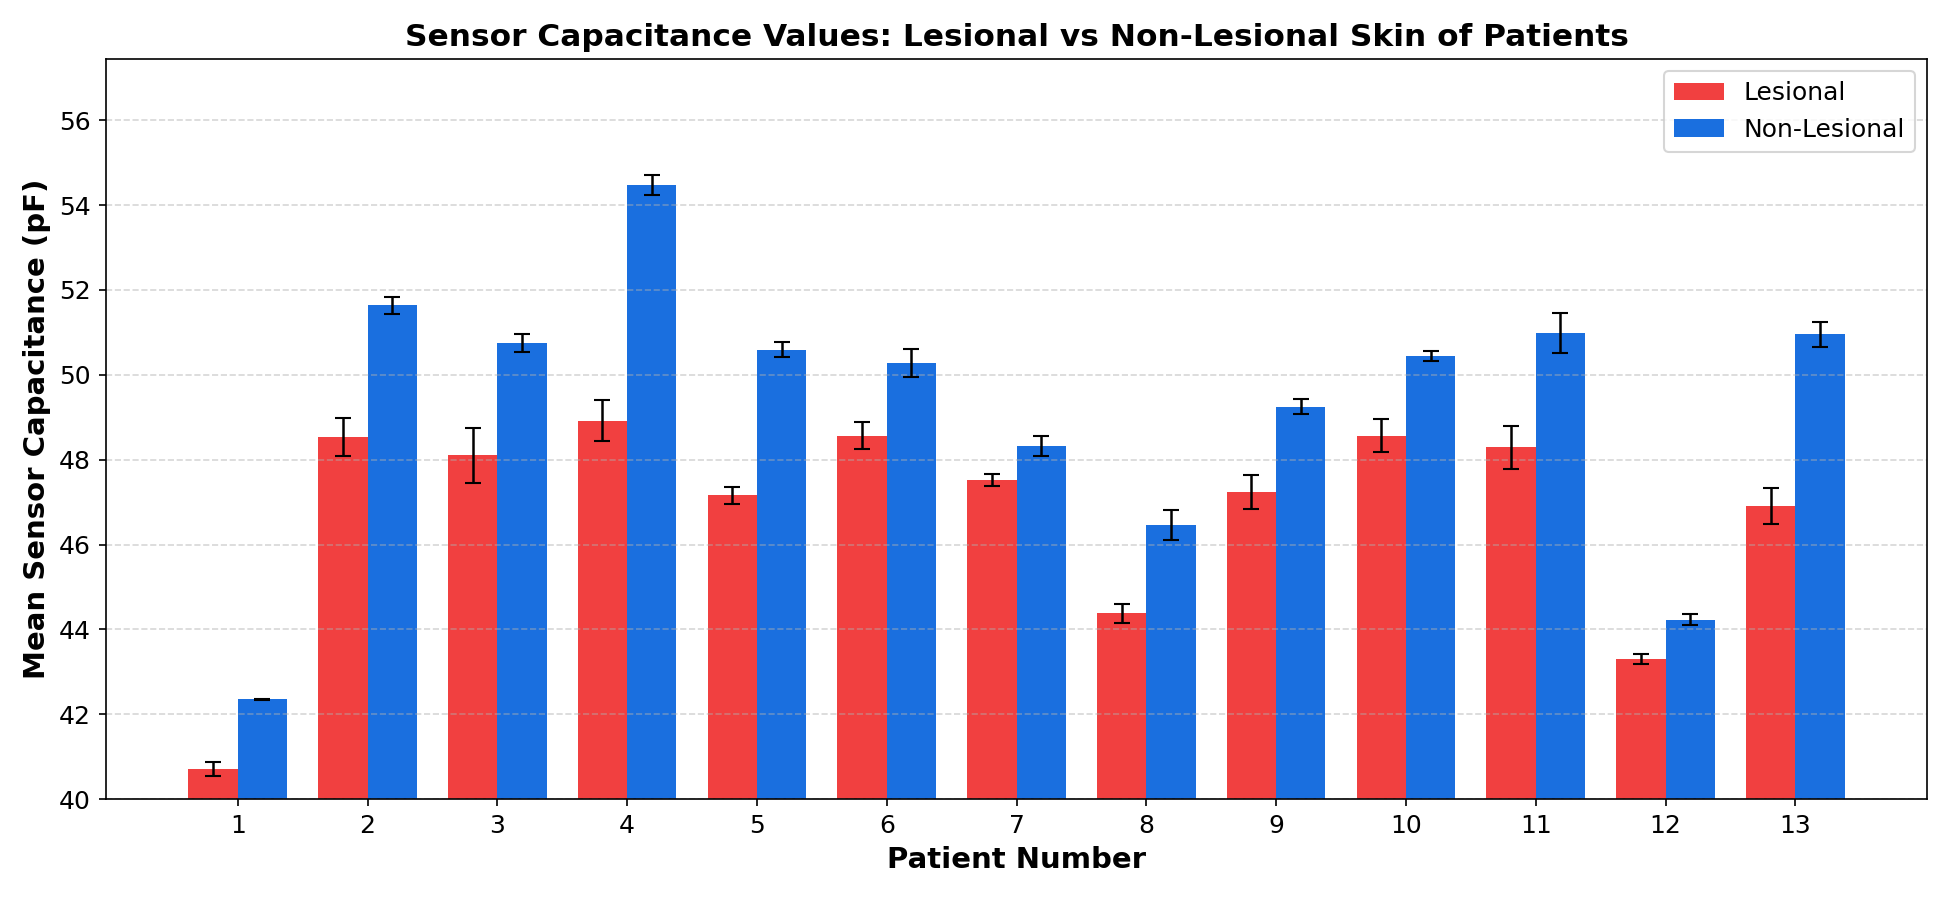
\includegraphics[width=\linewidth]{results/stage1_replication.png}%
  }{%
    \missingfig{\linewidth}{Stage 1: per-patient lesional vs.\ non-lesional capacitance}{python src/stage1\_replication.py}%
  }
  \caption{Per-patient mean capacitance for lesional and non-lesional sites
           (13 patients). Non-lesional exceeds lesional for every patient,
           replicating Todorov et al.\ \cite{todorov2025wearable} Fig.\ 9(a).
           Absolute levels vary by $\sim$10 pF across patients, explaining
           why a population-wide threshold cannot be defined.}
  \label{fig:stage1}
\end{figure}

Figure~\ref{fig:stage1} shows the per-patient mean capacitance for lesional and
non-lesional sites. Non-lesional capacitance exceeds lesional for every patient,
replicating the direction and per-patient ordering of Todorov et al.\ Fig.\ 9(a).
The advantage is consistent (2--5\,pF) but absolute levels vary by $\approx$10\,pF
across individuals (Patient 1 $\approx$40\,pF lesional vs.\ Patient 4 $\approx$49\,pF
lesional), confirming that a single population-wide decision threshold cannot
reliably distinguish lesional from non-lesional skin.

\subsection{Stage 2: Feature Importance}\label{sec:stage2}

\begin{figure}[t]
  \centering
  % Upload results/stage2_features.png to Overleaf, or run src/stage2_features.py locally
  \IfFileExists{results/stage2_features.png}{%
    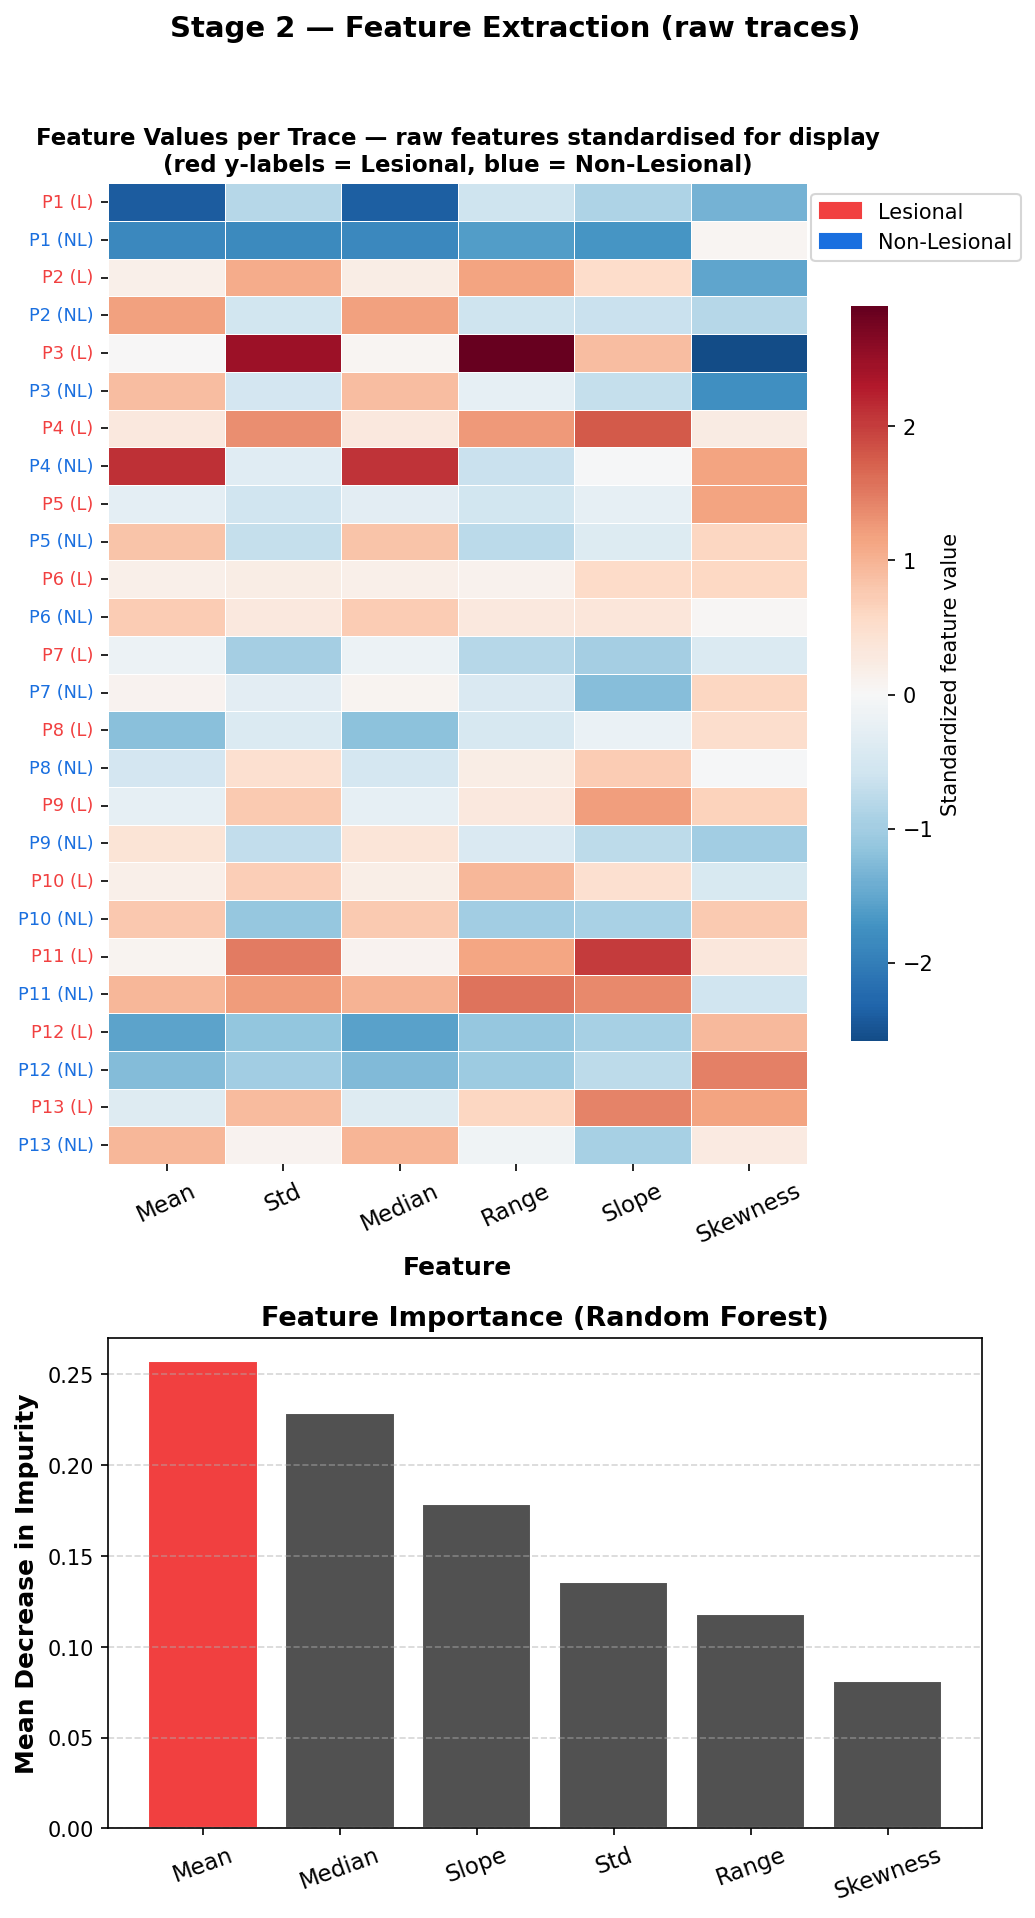
\includegraphics[width=\linewidth]{results/stage2_features.png}%
  }{%
    \missingfig{\linewidth}{Stage 2: RF feature importances + LOSO box plots}{python src/stage2\_features.py}%
  }
  \caption{Random Forest feature importances (top) and per-feature
           LOSO box plots (bottom) for all six statistical features
           extracted from raw 30-second traces ($N{=}26$).}
  \label{fig:stage2}
\end{figure}

\begin{table}[t]
  \caption{Random Forest feature importances on raw traces ($N{=}26$,
           \texttt{random\_state=42}).}
  \label{tab:feature_importance}
  \centering
  \begin{tabular}{clr}
    \toprule
    Rank & Feature   & Importance \\
    \midrule
    1    & Mean      & 0.257 \\
    2    & Median    & 0.229 \\
    3    & Slope     & 0.179 \\
    4    & Std       & 0.136 \\
    5    & Range     & 0.118 \\
    6    & Skewness  & 0.081 \\
    \bottomrule
  \end{tabular}
\end{table}

Table~\ref{tab:feature_importance} and Figure~\ref{fig:stage2} show Random Forest
feature importances on raw traces. All six features carry non-zero importance,
confirming that the full feature set is preserved by extracting from un-normalized
traces. Mean and Median rank first and second, directly reflecting the per-patient
capacitance advantage observed in Stage 1. Slope ranks third, indicating that
linear drift over the 30-second window differs between lesional and non-lesional
sites and provides additional discriminative information beyond level alone.

\subsection{Stage 3: Normalization Comparison}\label{sec:stage3}

\begin{figure}[t]
  \centering
  % MISSING: run `python src/stage3_normalization.py` to regenerate
  \IfFileExists{results/stage3_normalization.png}{%
    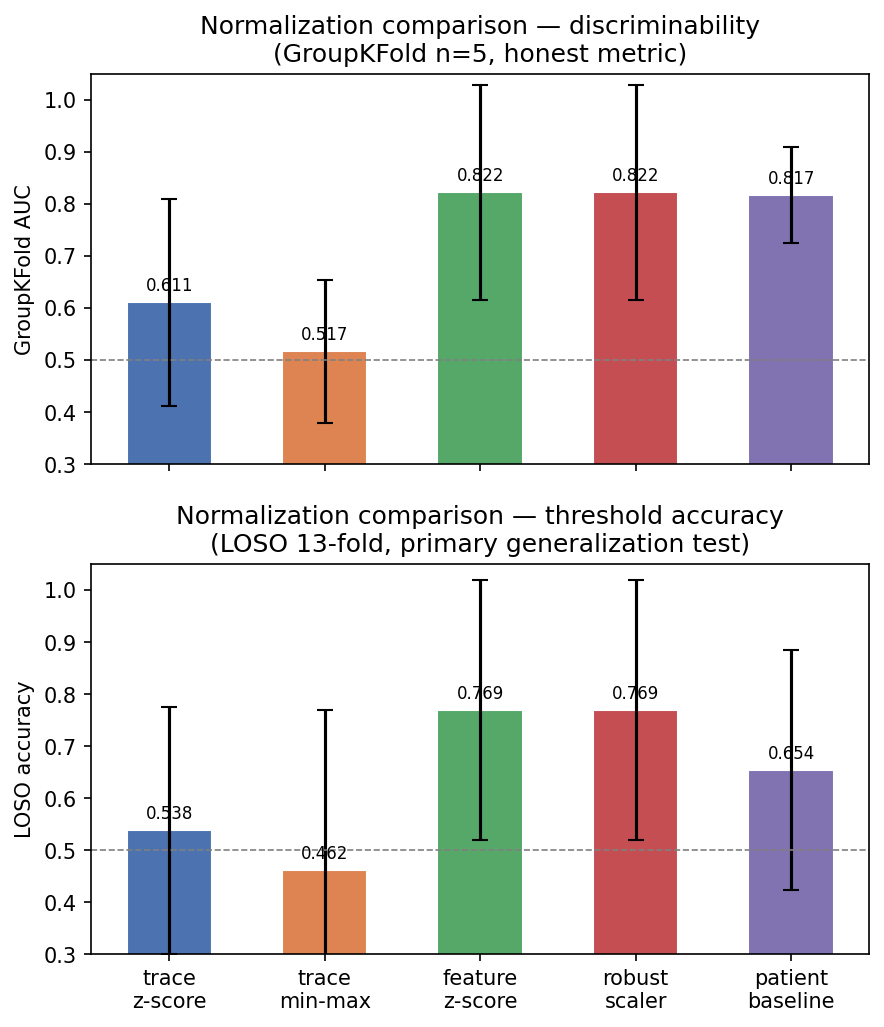
\includegraphics[width=\linewidth]{results/stage3_normalization.png}%
  }{%
    \missingfig{\linewidth}{Stage 3 normalization comparison bar chart}{python src/stage3\_normalization.py}%
  }
  \caption{GroupKFold AUC and LOSO accuracy for five normalization methods
           (LinearSVC). Feature z-score and RobustScaler tie on every metric;
           patient-baseline ``AUC 1.000'' collapses to 0.817 under GroupKFold,
           exposing it as a degenerate per-fold artefact.}
  \label{fig:stage3}
\end{figure}

\begin{table*}[t]
  \caption{Normalization comparison — LinearSVC, feature-level normalization,
           LOSO and GroupKFold ($n{=}5$). ``LOSO rank'' is a degenerate 2-sample-per-fold
           metric (= pairwise ranking fraction); use GKF AUC for honest
           discriminability comparison.  $\dagger$ = artifact, not a real AUC advantage.}
  \label{tab:normalization}
  \centering\small
  \begin{tabular}{lcccccc}
    \toprule
    Method
      & LOSO Acc
      & LOSO F1
      & LOSO Rank$^\dagger$
      & Pooled-LOSO AUC
      & GKF Acc
      & \textbf{GKF AUC} \\
    \midrule
    Feature z-score (primary)
      & $0.769 \pm 0.249$
      & $0.744 \pm 0.350$
      & 0.846
      & 0.781
      & $0.750 \pm 0.167$
      & $\mathbf{0.822}$ \\
    RobustScaler
      & $0.769 \pm 0.249$
      & $0.744 \pm 0.350$
      & 0.846
      & 0.793
      & $0.750 \pm 0.167$
      & $\mathbf{0.822}$ \\
    Patient baseline (fold-safe)
      & $0.654 \pm 0.231$
      & $0.462 \pm 0.444$
      & $1.000^\dagger$
      & 0.775
      & $0.700 \pm 0.113$
      & 0.817 \\
    Trace z-score
      & $0.538 \pm 0.237$
      & $0.410 \pm 0.396$
      & 0.769
      & 0.615
      & $0.583 \pm 0.105$
      & 0.611 \\
    Trace min-max
      & $0.462 \pm 0.308$
      & $0.308 \pm 0.402$
      & 0.462
      & 0.379
      & $0.433 \pm 0.178$
      & 0.517 \\
    \bottomrule
  \end{tabular}
\end{table*}

Table~\ref{tab:normalization} compares all five normalization methods. Feature-level
z-score and RobustScaler tie exactly on every metric, confirming that IQR-based
centering offers no practical advantage over mean/std centering at $N{=}26$.
Trace-level z-score degrades accuracy to 0.538 (near chance) because forcing
per-trace mean to zero destroys the mean and median features that carry the primary
signal. Patient-baseline centering achieves LOSO pairwise ranking of 13/13 but this
is a degenerate 2-sample-per-fold metric; under GroupKFold the advantage disappears
(0.817 vs.\ 0.822 for feature z-score). Feature-level z-score is adopted as the
primary normalization for all subsequent stages based on its higher threshold accuracy
(0.769) and GKF AUC (0.822).

\subsection{Stage 4: Window Length}\label{sec:stage4_results}

\begin{figure}[t]
  \centering
  % Upload results/stage4_window_length.png to Overleaf, or run src/stage4_window_length.py locally
  \IfFileExists{results/stage4_window_length.png}{%
    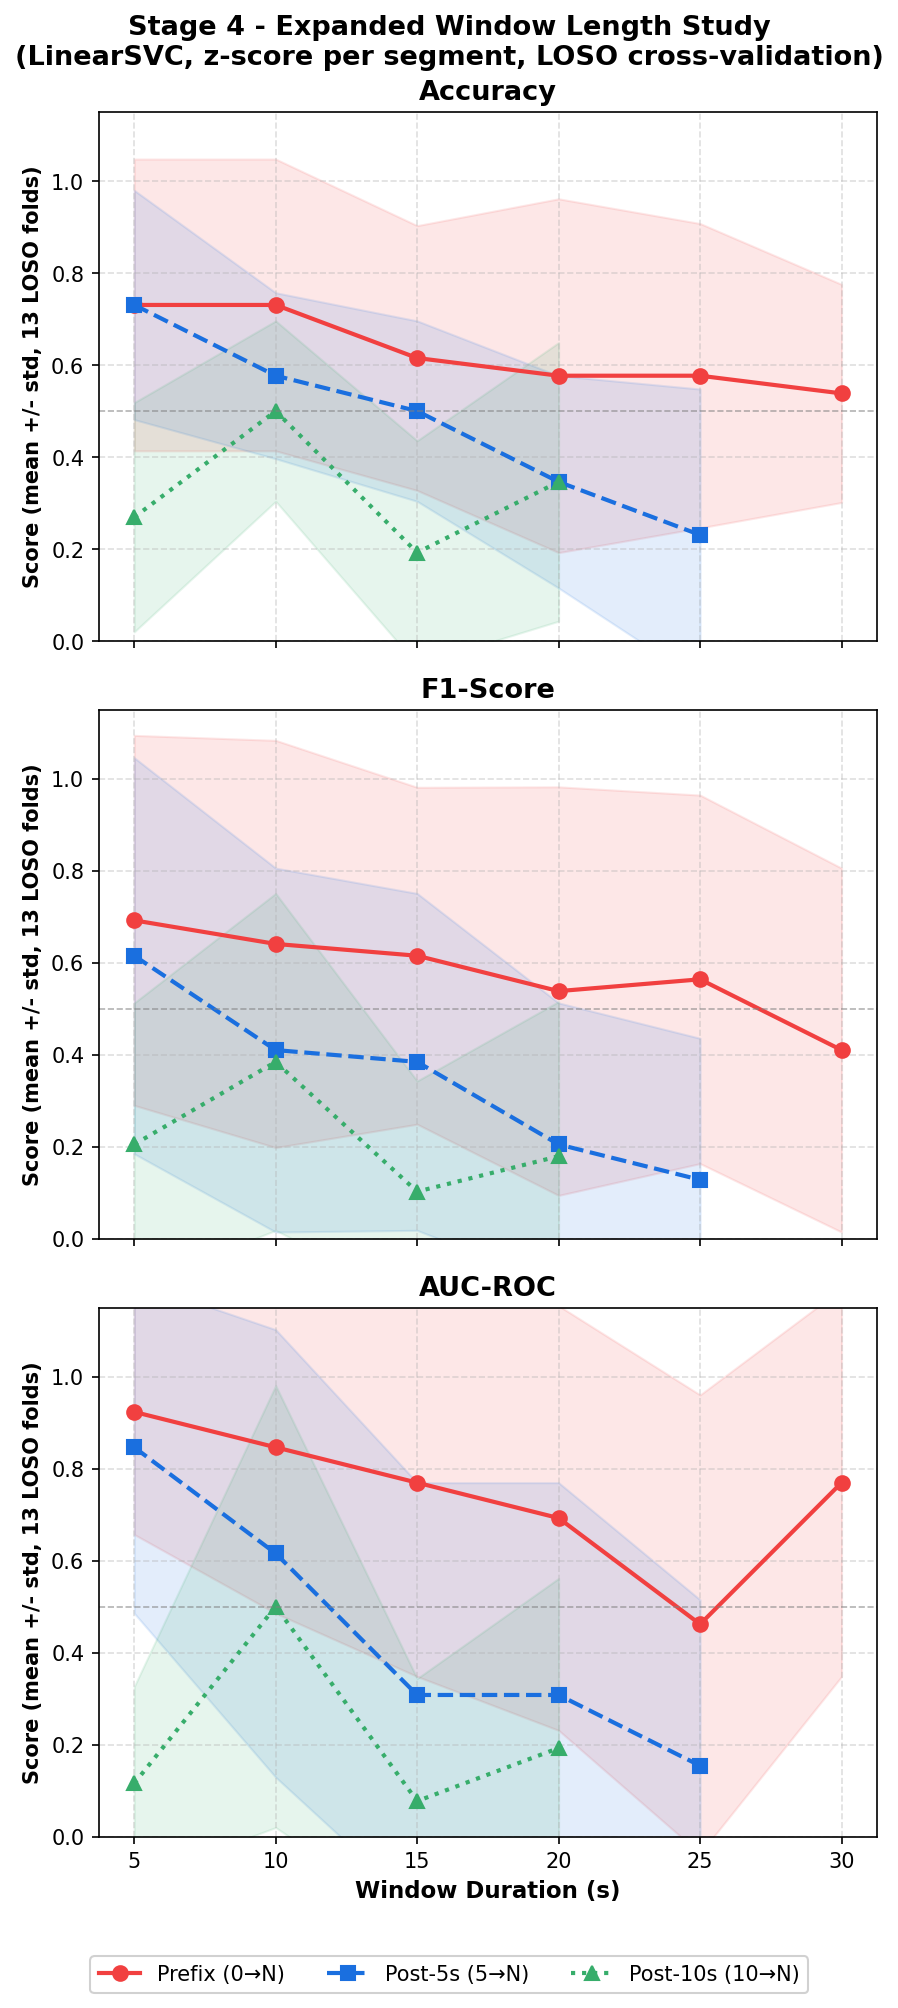
\includegraphics[width=\linewidth]{results/stage4_window_length.png}%
  }{%
    \missingfig{\linewidth}{Stage 4: window length LOSO AUC sweep}{python src/stage4\_window\_length.py}%
  }
  \caption{LOSO AUC (mean $\pm$ std) for prefix and post-settling window families.
           Performance degrades sharply past 10 s; post-10 s windows approach
           random due to backfill-constant segments in $\geq$3 patients.}
  \label{fig:stage4}
\end{figure}

\begin{table}[t]
  \caption{Selected window-length results (LinearSVC, feature z-score per segment,
           LOSO). Full table: \texttt{results/stage4\_window\_length.csv}.}
  \label{tab:window}
  \centering\small
  \begin{tabular}{llrr}
    \toprule
    Family & Window & Acc & AUC \\
    \midrule
    \multirow{3}{*}{Prefix (0$\to$N)}
      & 0–5\,s  & $0.731 \pm 0.317$ & $0.923 \pm 0.267$ \\
      & 0–10\,s & $0.731 \pm 0.317$ & $0.846 \pm 0.361$ \\
      & 0–30\,s & $0.538 \pm 0.237$ & $0.769 \pm 0.421$ \\
    \midrule
    Post-5\,s (5$\to$N)
      & 5–30\,s & $0.231 \pm 0.317$ & $0.154 \pm 0.361$ \\
    \midrule
    Post-10\,s (10$\to$N)
      & 10–30\,s & $0.346 \pm 0.303$ & $0.192 \pm 0.369$ \\
    \bottomrule
  \end{tabular}
\end{table}

Table~\ref{tab:window} and Figure~\ref{fig:stage4} show the window-length results.
The 0--5\,s prefix achieves the highest AUC (0.923) and performance degrades
monotonically as the window extends; post-settling windows are substantially
worse than equal-duration prefix windows at every length, with post-10\,s windows
approaching random classification. The root cause is a data-quality confound rather
than a clinical finding: patients S-02, S-03, and S-04 have genuine signal only in
approximately the first 10 seconds, so post-settling feature vectors for these
patients are uninformative constants. This confound prevents the experiment from
cleanly separating settling effects from signal duration. These results should not
be interpreted as evidence that shorter measurement windows are clinically superior.

\subsection{Stage 5: Evaluation Expansion}\label{sec:stage5_results}

\begin{table}[t]
  \caption{Evaluation metrics — LinearSVC, fold-safe patient-baseline
           normalization, full 30\,s traces.}
  \label{tab:eval}
  \centering\small
  \begin{tabular}{lccc}
    \toprule
    Method & Acc & F1 & GKF AUC \\
    \midrule
    LOSO (13 folds, primary)
      & $0.654 \pm 0.231$
      & $0.462 \pm 0.444$
      & — \\
    GroupKFold ($n{=}5$)
      & $0.700 \pm 0.113$
      & $0.651 \pm 0.146$
      & $0.817 \pm 0.092$ \\
    \bottomrule
    \multicolumn{4}{l}{\footnotesize
      Pooled-LOSO AUC = 0.775 (negative bias per \cite{airola2011comparison}).} \\
  \end{tabular}
\end{table}

Table~\ref{tab:eval} shows the evaluation results.
The model correctly ranks lesional above non-lesional for all 13 held-out patients
(pairwise ranking 13/13), directly supporting Todorov et al.'s intra-individual
tracking claim: trained exclusively on other patients, the model reliably identifies
which site is lesional for every unseen individual. LOSO threshold accuracy is 0.654,
reflecting the inability to define a reliable population-wide decision boundary ---
consistent with the inter-patient baseline variation observed in Stage 1.
GroupKFold AUC (0.817) and pooled-LOSO AUC (0.775) provide honest discriminability
estimates; their $\approx$0.04 gap is consistent with the negative bias of
pooled-LOO AUC \cite{airola2011comparison}. The accuracy--AUC gap (0.654 vs.\ 1.000)
provides evidence against data leakage: under oracle leakage, accuracy would also
approach 1.0.

\subsection{Stage 6A: CNN Track A vs.\ SVM}\label{sec:stage6_results}

\begin{figure}[t]
  \centering
  % MISSING: run `python src/stage6_cnn_trackA.py` to regenerate
  \IfFileExists{results/stage6_cnn_trackA.png}{%
    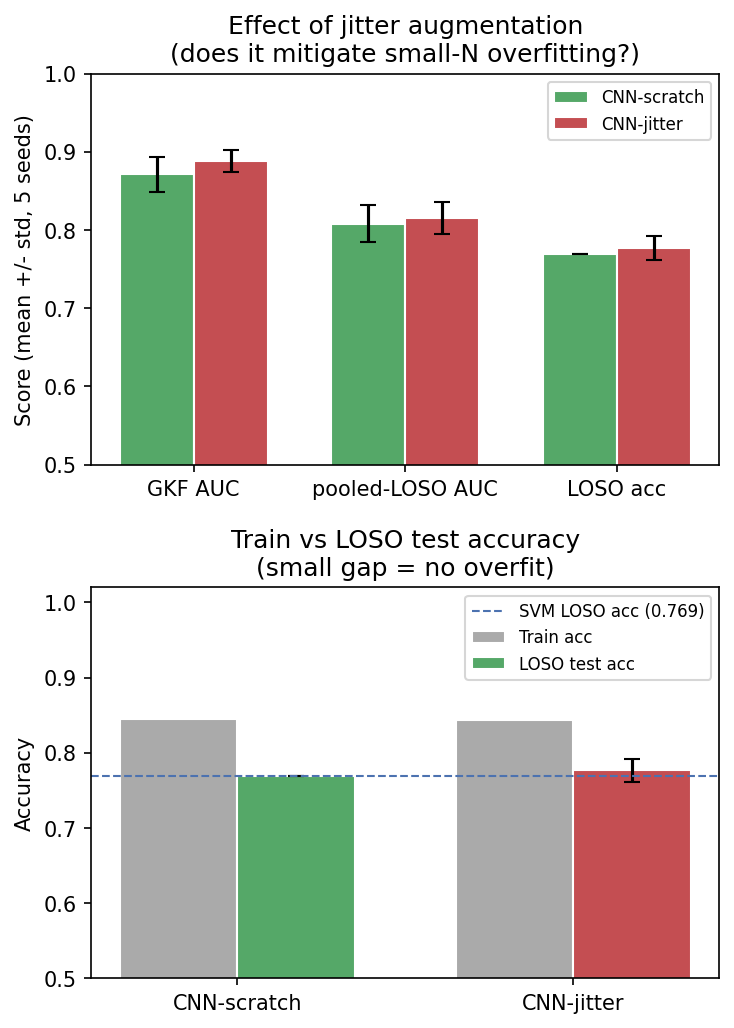
\includegraphics[width=\linewidth]{results/stage6_cnn_trackA.png}%
  }{%
    \missingfig{\linewidth}{Stage 6 Track A: CNN vs SVM training curve + metric comparison}{python src/stage6\_cnn\_trackA.py}%
  }
  \caption{Stage 6 Track A. \textit{Top:} training vs.\ test accuracy per
           LOSO fold (5 seeds; CNN-scratch and CNN-jitter). Small train–test
           gap confirms no over-fitting. \textit{Bottom:} GKF AUC comparison
           (CNN-scratch, CNN-jitter, SVM reference).}
  \label{fig:stage6}
\end{figure}

Figure~\ref{fig:stage6} and Table~\ref{tab:cnn_trackB} show the Track A results.
The CNN does not overfit: the train--test accuracy gap is 0.077 for CNN-scratch,
well below the pre-registered 0.20 trigger threshold. GroupKFold AUC of 0.871
edges above the SVM (0.822), and the jitter variant improves further to 0.889.
The small margin over the SVM despite access to the full raw trace --- rather than
six handcrafted features --- suggests both models converge to the same underlying
representation. Global Average Pooling computes a weighted mean across the time
dimension, so the CNN effectively rediscovers the mean capacitance level that ranks
first in the Stage 2 Random Forest importance. Jitter augmentation offers only
marginal improvement (0.018 GKF AUC) because there is no waveform complexity to
regularize: the discriminative signal is a level difference, not a shape.

\subsection{Stage 6B: Transfer Learning (Track B)}\label{sec:stage6b_results}

\begin{figure}[t]
  \centering
  % Upload results/stage6_cnn_trackB.png to Overleaf, or run src/stage6_cnn_trackB.py locally
  \IfFileExists{results/stage6_cnn_trackB.png}{%
    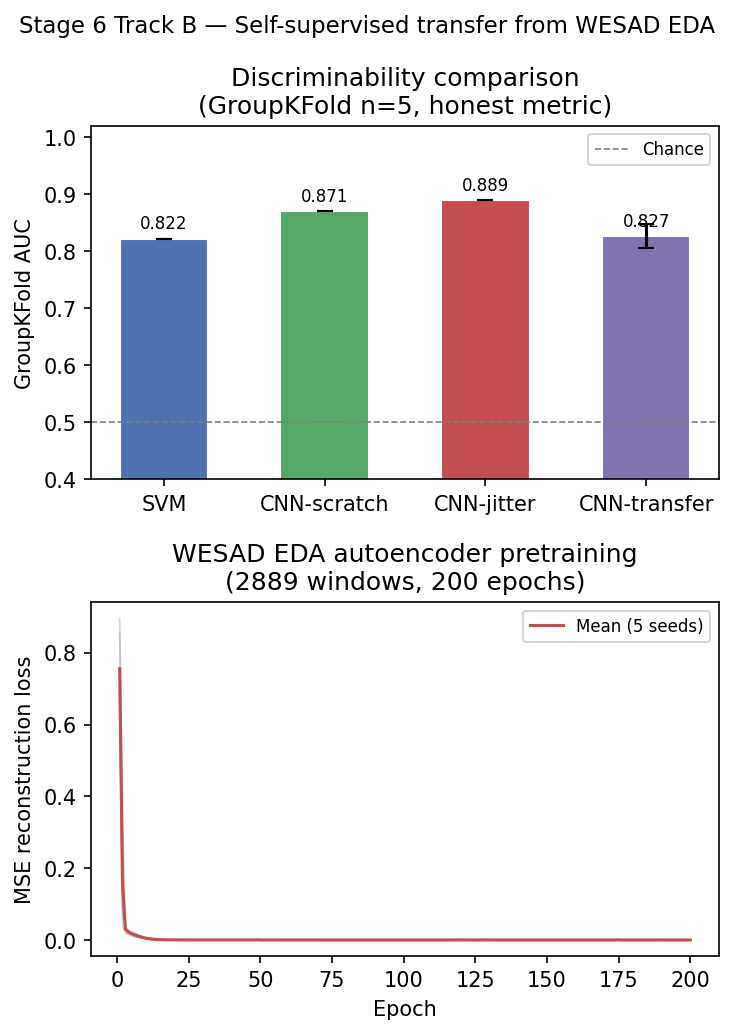
\includegraphics[width=\linewidth]{results/stage6_cnn_trackB.png}%
  }{%
    \missingfig{\linewidth}{Stage 6 Track B: transfer CNN vs.\ Track A + SVM}{python src/stage6\_cnn\_trackB.py}%
  }
  \caption{Stage 6 Track B: self-supervised pretrained CNN (WESAD EDA, frozen
           conv) vs.\ Track A baselines. GKF AUC 0.827 falls below CNN-scratch
           (0.871) and CNN-jitter (0.889), indicating that EDA pretraining does
           not improve IDC classification at $N{=}26$.}
  \label{fig:stage6b}
\end{figure}

\begin{table}[t]
  \caption{Full model comparison — Stages 6A and 6B. Values are mean$\pm$std
           over 5 random seeds.  Track B GKF AUC (0.827) falls below both
           Track A variants despite domain-adjacent pretraining.}
  \label{tab:cnn_trackB}
  \centering\small
  \begin{tabular}{lcccc}
    \toprule
    Model & Train Acc & LOSO Acc & GKF AUC & Pooled-LOSO \\
    \midrule
    CNN-jitter
      & $0.844 \pm 0.002$
      & $0.777 \pm 0.015$
      & $\mathbf{0.889} \pm 0.014$
      & $0.815 \pm 0.021$ \\
    CNN-scratch
      & $0.846 \pm 0.001$
      & $0.769 \pm 0.000$
      & $0.871 \pm 0.022$
      & $0.808 \pm 0.024$ \\
    CNN-transfer
      & $0.726 \pm 0.036$
      & $0.715 \pm 0.039$
      & $0.827 \pm 0.022$
      & $0.773 \pm 0.008$ \\
    SVM (ref.)
      & —
      & 0.769
      & 0.822
      & 0.781 \\
    \bottomrule
    \multicolumn{5}{l}{\footnotesize Track B LOSO rank = $0.985 \pm 0.031$; Train–test gap = 0.011.} \\
  \end{tabular}
\end{table}

Table~\ref{tab:cnn_trackB} and Figure~\ref{fig:stage6b} show the full four-model
comparison. The transfer CNN (Track B) achieves GKF AUC 0.827, above the SVM (0.822)
but below both from-scratch variants (0.871 and 0.889). The train--test gap of 0.011
confirms that the frozen encoder is stable, but the pretrained features offer no
discrimination advantage over features learned directly from the IDC data. Across
all models, jitter augmentation (Track A) achieves the highest GKF AUC (0.889);
neither transfer learning nor jitter changes the qualitative conclusion that the
discriminative signal is the per-site mean capacitance level.

% ============================================================
\section{Discussion}\label{sec:discussion}

\subsection{Interpreting the LOSO AUC}
With exactly one lesional and one non-lesional test sample per LOSO fold,
\texttt{roc\_auc\_score} can only return 0 (incorrect ranking) or 1 (correct
ranking), so the mean across 13 folds equals a pairwise ranking accuracy, not a
graded ROC area. ``LOSO AUC 1.000'' means the model ranked lesional above
non-lesional for every held-out patient --- a meaningful finding --- but it cannot
be compared to AUC values computed over larger test sets in the literature.
Genuine discriminability is measured by GroupKFold AUC (0.822 for the SVM, 4--6
test samples per fold) and pooled-LOSO AUC (0.775). The accuracy--AUC gap (0.654
vs.\ 1.000) provides evidence against oracle data leakage: if training data were
contaminated with test-patient information, accuracy would also approach 1.0. The
absence of leakage was further verified programmatically: in 0 of 13 LOSO folds
did the held-out patient's data contribute to its own normalization baseline.

\subsection{Why the CNN Ties the SVM}
The most informative result in Stage 6 is not that the CNN edges the SVM, but why
the margin is so small despite the CNN having access to the full raw signal rather
than six handcrafted features. Global Average Pooling reduces the 1D feature map
to a scalar per channel by averaging across time, effectively computing a weighted
mean of the trace. The CNN therefore converges to the same representation as the
SVM's top feature (trace mean), learned end-to-end rather than engineered. A model
that sees strictly more information yet only marginally exceeds a simpler model
using mean capacitance alone is strong evidence that the discriminative signal in
this corpus is a level difference, not a temporal pattern. Any architecture with an
implicit or explicit mean-pooling operation will likely reach the same performance
ceiling on this dataset.

\subsection{Data Quality Confound}
The window-length experiment cannot answer its intended question because a subset
of traces contain forward-filled constants beyond approximately the first 10
seconds. For patients S-02, S-03, and S-04 (and possibly others), any feature
extracted from the post-10\,s portion of the trace is determined entirely by the
last genuine sample, producing near-zero variance feature vectors. Post-settling
windows yield near-random classification not because later samples carry no
physiological signal, but because those samples simply do not exist for a
substantial fraction of the dataset. Correctly interpreting the settling analysis
would require first identifying which patients have complete 30-second genuine
signals, then restricting the comparison to those patients only. This is left as
future work.

\subsection{Limitations}
Several limitations bound the scope of these findings. At $N{=}13$ patients,
fold-to-fold variance in LOSO evaluation is very high (accuracy std 0.231); any
reported mean metric could shift substantially with a small change in the patient
sample, and all results should be treated as indicative rather than definitive.
The Corneometer correlation analysis (Stage 7) was not performed, leaving the
relationship between IDC-derived features and established clinical skin hydration
measures uncharacterized; TEWL measurements are excluded due to limited data
availability. The TinyCNN architecture represents a single design point with no
hyperparameter search. Track B used strictly frozen convolutional layers; a
two-phase strategy (pretrain, then gradually unfreeze and fine-tune) was not
explored and may yield a different outcome. Finally, the LOSO binary-fold AUC
is not comparable to AUC values in multi-sample cross-validation studies and
should not be cited as such.

\subsection{Why Transfer Learning Did Not Help}
Track B GKF AUC (0.827) falls below the from-scratch CNN (0.871) despite pretraining
on a domain-adjacent 1D skin signal. The most plausible explanation is a fundamental
sensor physics mismatch: EDA measures ionic conductance of eccrine sweat glands,
while IDC capacitance measures dielectric permittivity of the stratum corneum
barrier. Both are 1\,Hz skin-surface measurements, but their signal dynamics,
amplitude scales, and physiological drivers differ substantially. The self-supervised
reconstruction objective encourages the encoder to capture EDA-specific low-frequency
drift and motion artifacts that are not discriminative in IDC capacitance traces.
The from-scratch CNN, unconstrained by any prior signal representation, converges
directly to the IDC mean-level feature. Freezing the conv layers prevents this
adaptation. Future work could explore two-phase transfer (pretrain then unfreeze),
or use a domain-closer pretraining source if a larger IDC-specific dataset becomes
available.

% ============================================================
\section{Conclusion}\label{sec:conclusion}
This study demonstrates a proof-of-concept machine learning pipeline capable of distinguishing lesional from non-lesional skin in AD patients using highly constrained wearable IDC sensor data. By replicating established findings that non-lesional capacitance consistently exceeds lesional capacitance at an individual level, we confirm that a single population-wide decision boundary is ineffective due to significant baseline variations across patients. Instead, intra-individual tracking proves highly reliable: a baseline LinearSVC model successfully ranked lesional severity correctly for 13 out of 13 held-out patients, achieving a GroupKFold AUC of 0.822.  While end-to-end deep learning via a 1D CNN marginally outperformed the traditional statistical approach (GKF AUC 0.871), an analysis of its architecture confirms that the discriminative signal lies almost entirely in the mean capacitance level rather than in intricate temporal dynamics. Furthermore, efforts to mitigate data scarcity through self-supervised transfer learning on domain-adjacent EDA signals proved unsuccessful (GKF AUC 0.827), highlighting how the physical gap between measuring eccrine sweat conductance versus stratum corneum permittivity limits knowledge transfer. Our analysis of measurement duration also exposed critical dataset artifacts, emphasizing the need for rigorous data hygiene in future wearable studies to prevent confounding results. Ultimately, while this work validates the potential of continuous IDC monitoring for personalized AD tracking, transitioning from proof-of-concept to robust clinical deployment will require significantly larger, artifact-free datasets.

% ============================================================
\begin{acks}
AI tools (Claude) were used for concept explanation, literature search, code
guidance, and report generalization. Experimental design, research questions,
and scientific conclusions were determined by the author. All AI-generated
code was reviewed, tested, and modified.
\end{acks}

% ============================================================
\bibliographystyle{ACM-Reference-Format}
\bibliography{references}

\end{document}
